\chapter{Motivation}

In this chapter we will introduce the very motivation of this work. From medical point of view, this work focuses on a medical condition known as intracranial hemorrhage. We will adduce the elementary facts about this condition for more comprehensive understanding of the whole problematic. Furthermore, an overview of standard approach to the process of diagnostics will be presented.

\section{Intracranial hemorrhage}
Intracranial hemorrhage, commonly referred to as ICH, is a serious and potentially deathly health condition. This type of hemorrhage poses any type of bleeding present within the fixed intracranial vault \cite{intracranial1}. The most common causes of intracranial hemorrhage are a traumatic brain injury as well as spontaneous appearance, due to a vascular malformation, which stands for a disease of the vessel \cite{intracranial2}. If not treated promptly, the hemorrhage can subsequently account for even more serious conditions, such as coma, seizures or stroke \cite{intracranial2}. Strokes can be categorized as hemorrhagic - caused by an intracranial bleeding, and ischemic - result of a blockage in an artery supplying blood to the brain. As stated in the book of Urden er al. \cite{ICHbookstats}, 13\% of all strokes in the United States yearly are hemorrhagic strokes and 87\% are ischemic strokes. Although hemorrhagic strokes occur less frequently, their mortality rate is much higher, with 37\% to 38\% of such cases resulting in death within the first month. After cardiovascular diseases, cancer and chronic respiratory diseases, stroke is the fourth leading death cause in the United States \cite{ICHbookstats}. The number of deaths can be greatly decreased with accurate and precocious diagnosis.

\section{Types of hemorrhage}
There are five most common subtypes of intracranial hemorrhage, varying in the region in which they appear in the intracranium \cite{ICHsubtypes-CT, imagingICH}. These subtypes are intraparenchymal, intraventricular, subarachnoid, subdural and epidural hemorrhage. Figure 2.1 presents examples of CT findings of each of the subtypes respectively.

\begin{figure}[h]
\begin{centering}
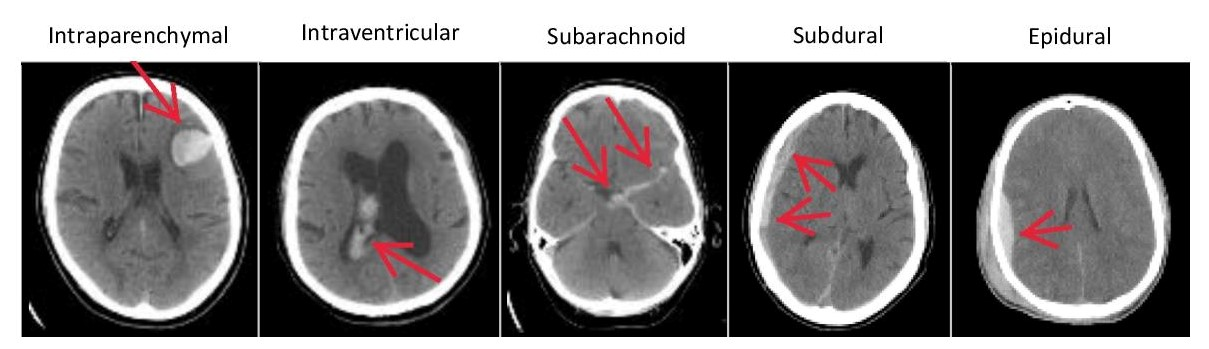
\includegraphics[width=14cm]{assets/images/subtypes}
\par\end{centering}
\caption{Five intracranial hemorrhage subtypes \label{fig:subtypes}}
\end{figure}

The symptoms of the patient and the severity of the bleeding is dependant largely on the subtype. Intraparenchymal hemorrhage is bleeding inside the brain tissue itself, classically centered in the basal ganglia \cite{imagingICH}. It mostly affects patients in the age category from sixty to seventy years. Intraventricular hemorrhage occurs, when the bleeding extends into the ventricles. They are quite uncommon, but can have significantly high mortality rate \cite{neuroimagingInTraumaticImageing}. The third subtype is subarachnoid hemorrhage, which affects the region between the arachnoid and the pia mater. Bleeding in the tissue surrounding the brain is reffered to as extra-axial. Examples of such bleedings are the subdural and epidural subtypes.

\section{Diagnostics}
The current standardized method for diagnosis of intracranial hemorrhage is non-contrast head computer tomography (CT) scanning \cite{imagingICH}. The interpretations of the CT scans are provided by radiologists, however in emergency situations, where quick evaluation is needed, scans are often reviewed by less experienced junior radiologists or attending physicians. A few studies have shown that this can lead to potential misinterpretations, resulting in false diagnosis and even negative consequences on patient's medical condition.  \cite{residentEval, overnightCTinterpret}. In their study, Strub et al. \cite{overnightCTinterpret} concentrated on detecting the rate and cause of errors in interpreting CT scans made by radiology residents, while on call during night shifts. As a result, they stated that misinterpretations of intracranial hemorrhage in head CT scans occur most frquently with subdural and subarachnoid hemorrhage sub-types, in 39\% and 33\% respectively. Overall, out of 22 590 patients' examinations overnight, 1037 discrepancies ensued, 147 of which were cases of intracranial hemorrhage.

Therefore, the motivation of this work is to propose and implement an algorithm, which could potentially work as an aid-tool to intracranial hemorrhage detection and sub-type classification. With such system, the whole process of interpreting CT scans could become more accurate and less faulty.